\section{Hardware Implementation}
\label{sec:implementation}

A possible hardware implementation of the \disr{} algorithm will be
described in this section.  Before enter in to detail of  \disr{}
architecture,  an idea of node structure tailored for this particular
scenario, can be found depicted in Fig.~\ref{fig:node_structure}. In
particular, such node should have the following foundamental elements:

\begin{itemize}%----Start Itemize------

\item \textbf{I/O Buffers-Trasceivers:} These elements, one for
each port,  are responsible of data transmission between neighbours
nodes. The packets received or sent are stored in specifieds buffers
named input and output buffers respectivelly.

\item \textbf{Switch Matrix:} Driven by a switch controller, enables the
reciprocal connections beetween the devices inside the node. Before
the creation of segments, such controller receives information from
\disr{} block.  After this phase, the switch controller will be driven by
the block wich implements the routing algorithm. The Switch matrix is
essentially a series of multiplexers and demultiplexers.

\item  \textbf{Processing Element (PE):} Is strictly related to the node
functionality  and role inside a given network, e.g. being a
computation or storage node.

\item \textbf{\disr{}-Routing:} The \disr{} block contains all the hardware, control
logic and configuration registers, related to the implementation of the
proposed approach. The routing algorithm receives information
from \disr{}  wich indicates the status of the segments that interests a
particular node. The routing operation will take in account of these
informations in order to perform a deadlock-free routing. Both Routing
and \disr{} are connected to the switch matrix in order to receive
packets from the input buffer. Since the packets are processed one at
a time, a specific arbiter should be present within the switch matrix
controller. 

\end{itemize}%------End Itemize------

\begin{figure}
  \centering
  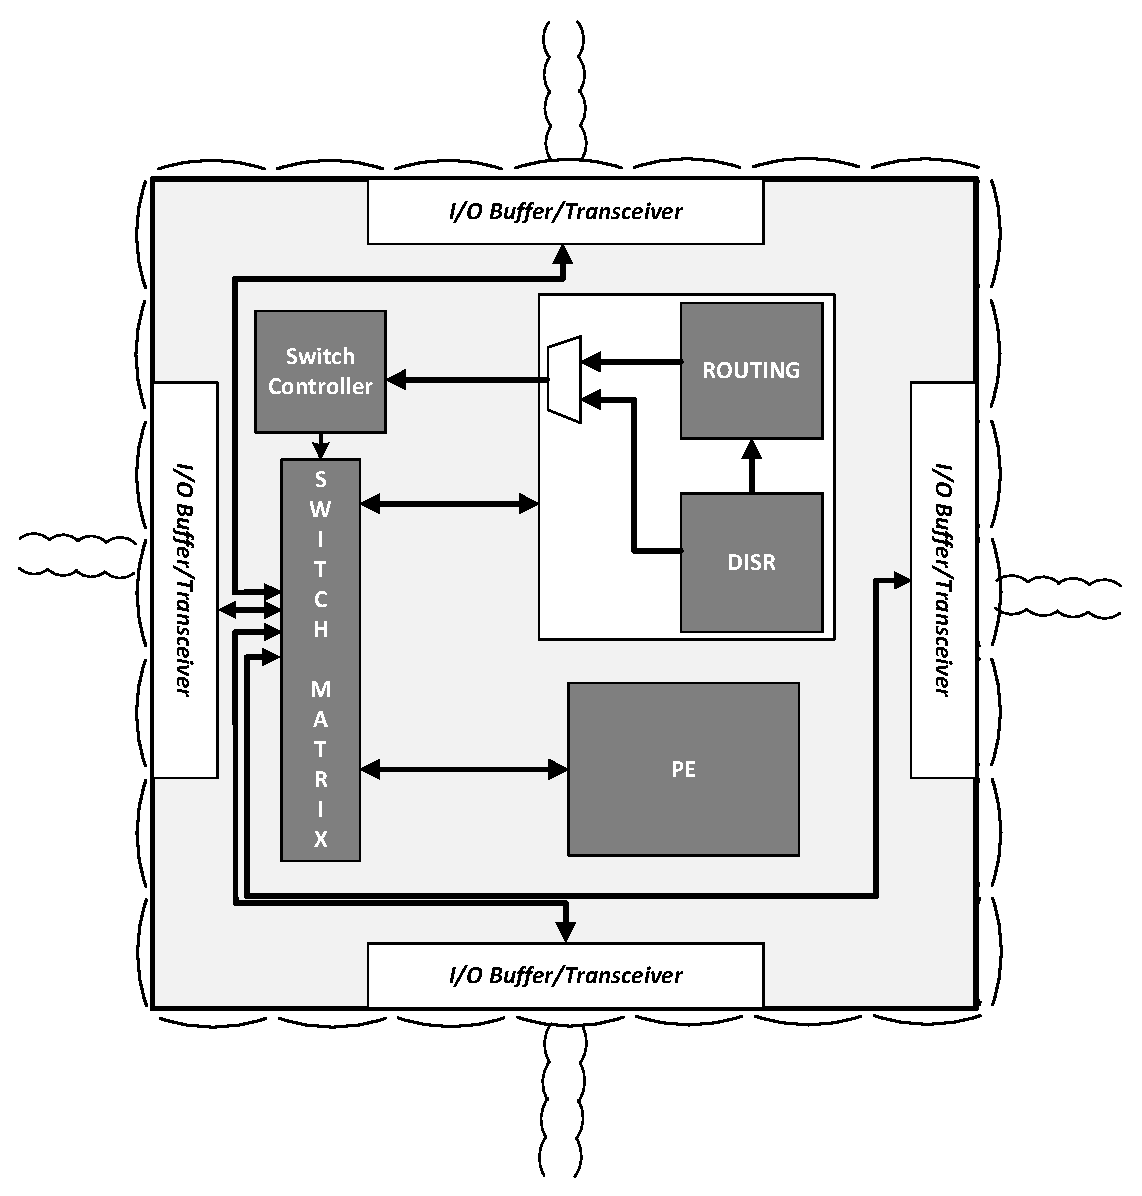
\includegraphics[width=0.45\textwidth]{pictures/node_structure.eps}
  \caption{A possible node structure tailored for a DNA nanonetwork.}
 \label{fig:node_structure}
\end{figure}
%--------------------------------------------------------------------
\subsection{\disr{} Architecture}
\label{ssec:disr_architecture}

\begin{figure}
  \centering
  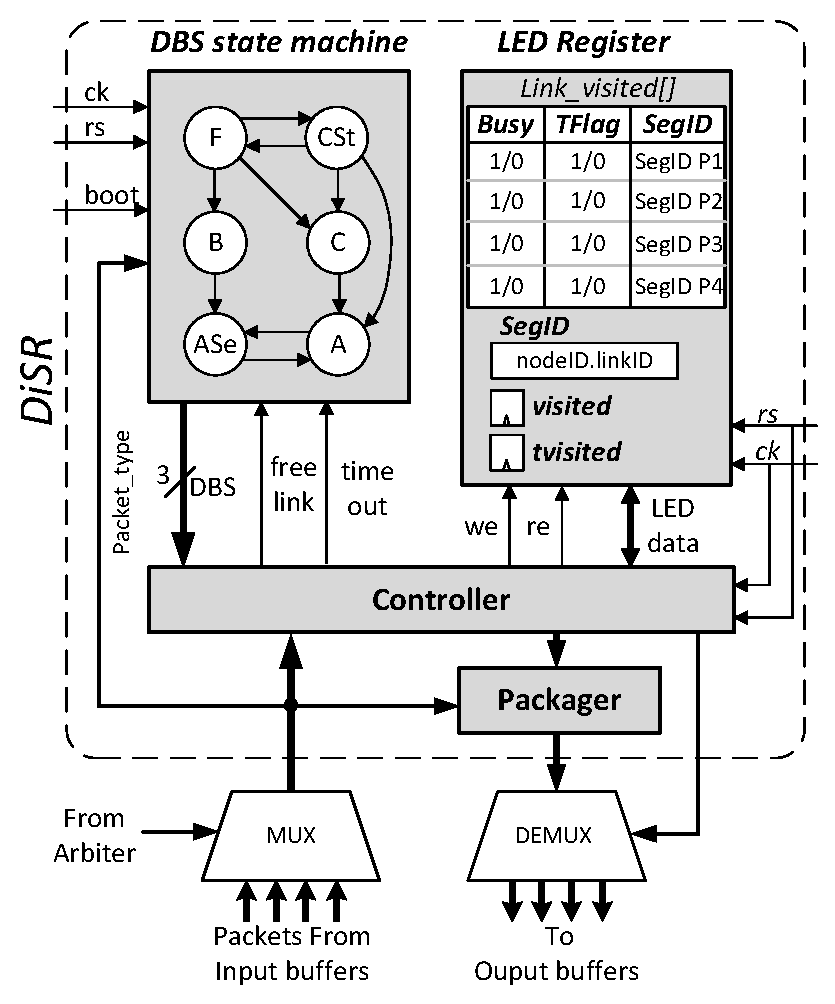
\includegraphics[width=0.40\textwidth]{pictures/disr_rtl_updated.eps}
  \caption{\emph{\disr{}} block architecture.}
 \label{fig:implementation}
\end{figure}

To give a basic estimate of the overhead needed we will focus on \disr{}-
specific components, that is, the control logic and configuration
registers needed to implement \disr{}. In Figure~\ref{fig:implementation}
is shown a sketch of the  architecture, which mainly consist in the
following building elements:

\begin{itemize}

	\item \textbf{DBS block:} 
	It takes trace of the DBS state machine, 
	consisting of a 3-bit register (to cover six DBS values) and the 
	required combinational logic. This block receives signals from 
	stored packets  in order to decode the packet type, and from 
	the control circuitry to change its status.
	The bootstrap node is selected by setting the boot signal to high
	during the initialization phase. 

	\item \textbf{LED registers:} 
	A set of registers store the \emph{LED} listed in the
	section~\ref{sec:disr_concepts}.  In particular, in the
	link\_visited[] table, can be pointed out the presence of two  
	particular registernamed \emph{tflag} and \emph{busy}.  The Latter
	is used to indicate if a specific port is alredy visited or tvisited and
	the former indicates specifically if the node is visited or tvisited.

    \item \textbf{Control circuitry:}
    This circuitry decodes the the      incoming packet, the LED
	registers and the DBS,     updating them when required. This block
	drives the LED register   to store or, to read the LED data
	according with     \emph{write enable (WE)} or \emph{read enable (RE)}
	signals. Then, the resulting \emph{Ctrl-Out} drives the other
	communication resources for actuating the \disr{} routing operation.

	\item \textbf{Packager:}
	Essentially is a set of registers and multiplexers. Starting from
	an incoming packet stored in the input buffer, it updates the
	content of the packet before the retransmission to   a destination
	node.  In some cases, this circuitry build the packet from the
	scratch.  For example this happens when a node is bootsrap and for
	the first time it should inject a
	\emph{strating\_segment\_request}. In Fig.~\ref{fig:packager} is
	shown the architecture of such packager block. When a packet is
	created for the first time, the multiplexers driven by the
	controller select the information coming from the internal node
	such as the \emph{soruce\_ID}. In this situation the TTL field
	should be resetted to its initial value and the \emph{segment\_ID}
	is composed by the node ID and by the output port identification 
	number.

\end{itemize}

While the elements mentioned above are part of the \disr{} circuitry, 
the other devices depicted in Fig.~\ref{fig:implementation} like the 
multiplexer and demultiplexer are implemented outside \disr{}.
In particular, such components will be within the switch matrix 
(refers to the Fig~\ref{fig:node_structure}).

\begin{figure}
  \centering
  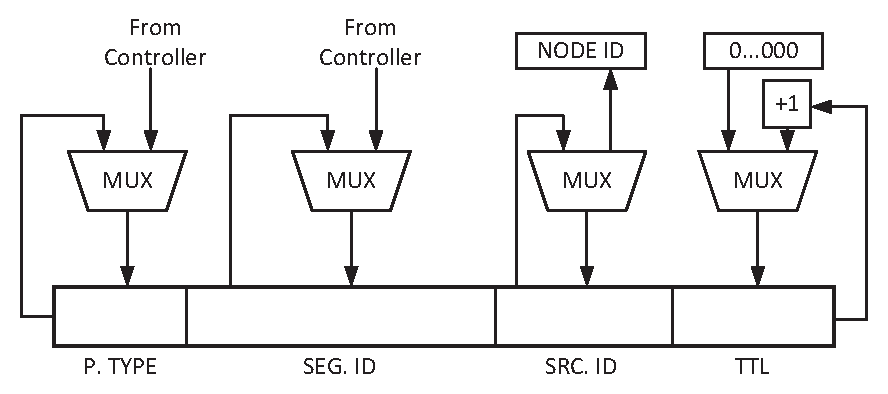
\includegraphics[width=0.40\textwidth]{pictures/packager.eps}
  \caption{Packager block}
 \label{fig:packager}
\end{figure}

\begin{figure}
  \centering
  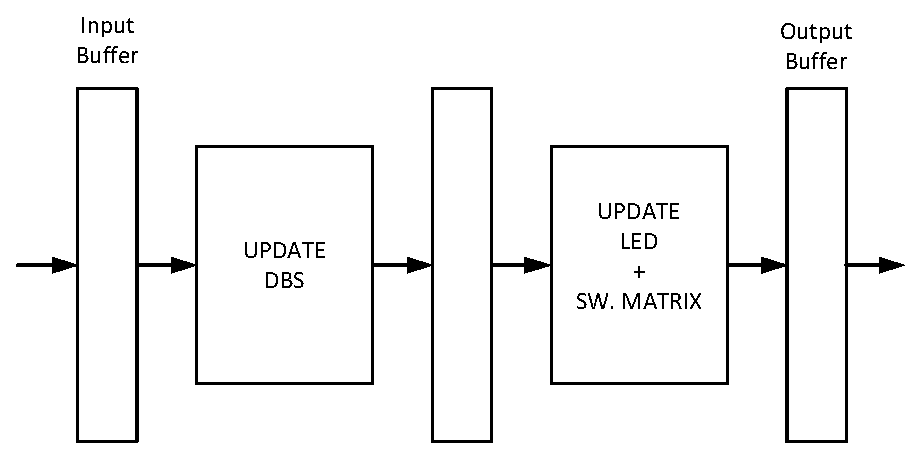
\includegraphics[width=0.40\textwidth]{pictures/pipeline.eps}
  \caption{Pipeline description of \disr{} operations}
 \label{fig:pipeline}
\end{figure}

Each just described building block, reacts with the rising edge  of
the\emph{clock signal}. An asynchronous system \emph{reset} signal is
also present for restoring all registers to their default values. When
this last signal is set, the DBS state machines for each network's
node are set as \emph{Free}.  
In Fig.~\ref{fig:pipeline} is described the pipeline structure of the
\disr{} architecture. The packet incoming from the neighbours node, or
locally generated will be send to the DBS state machine in order to te
ensure the status commutation. While the DBS update its state,  in the
next clock cycle the control circuitry will update the Led status and
will drive the sitch matrix in order to send eventually the packets to
the  right output buffer.
%--------------------------------------------------------------------
\subsection{Synthesis results}

As discussed above, one of the main design challenge of DNA Self-
Assembled systems is the limited resource available to implement both
computations and routing decisions for each node. Assuming a budget of
$10^4$ CNFETs for each network's node~\cite{liu_jetcs}  we estimated
the required resources for implementing the entire \disr{} block. The RTL
description of the circuitry described in the last section (with an
hardware description language)  of the \disr{} circuitry has been written
and synthesized at gate-level using \emph{Synopsys Design Compiler} with 
a generic technology library (GTECH).
Considering the specific layout of each single logic elements  (NAND,
full-adder, latch etc.), it has been possible to get a rough estimate
of the number of transistors necessary to implement the \disr{} logic.
Figure~\ref{fig:synthesys} shows the results of synthesis in terms of
number of devices (CNFETs) versus the number of network nodes while
the network scales up from $10\times10$ to $100\times100$ nodes.

\begin{figure}
  \centering
  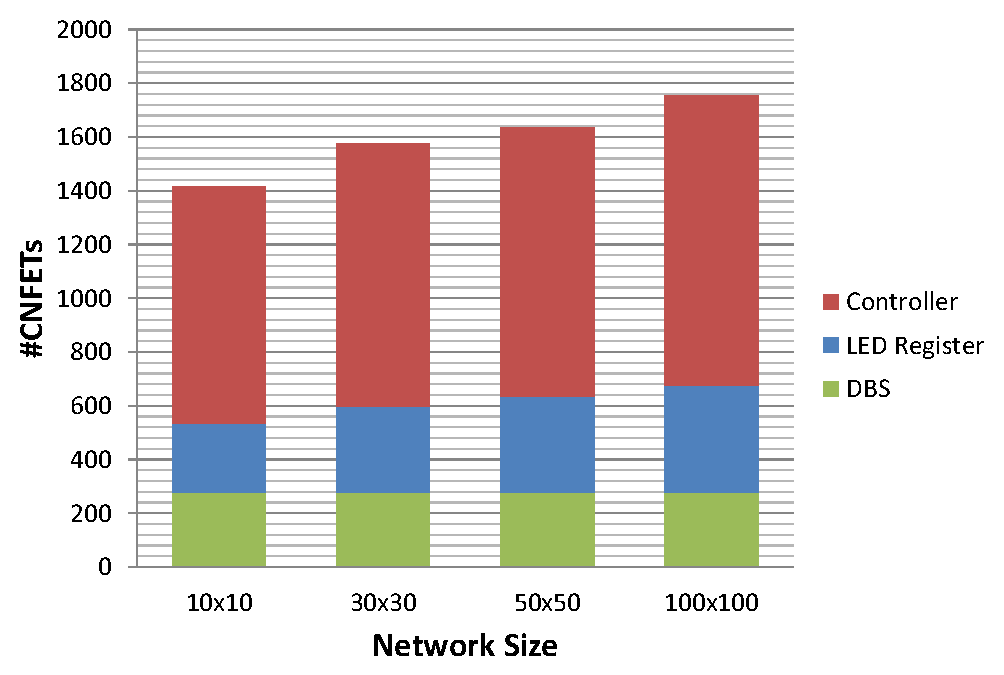
\includegraphics[width=0.50\textwidth]{pictures/synthesis.eps}
  \caption{Number of network's node (N) vs number of CNFETs necassary to implement
  the \disr{} circuitry.}
 \label{fig:synthesys}
\end{figure}

In particular, observing the Figure~\ref{fig:synthesys} can  be
pointed out that the proposed implementation occupies about 17,5\% of
the node budget. In particular the main contribution is due to the
controller circuitry followed by LED registers. Further, more than the
absolute number of devices itself, it is interesting to observe that
the circuitry complexity which implements the \disr{} algorithm increases
with a slowly growing trend.   An intuitive explanation of this is the
relatively simple logic of \disr{}, whose behaviour is almost code on
scalable storage structures. For example, the number of registers
implementing the \emph{link\_visited[]} and \emph{link\_tvisited[]}
table follow the logarithmic function $N_{reg}=N_{port} \cdot
log_2(N)$ where \emph{Nport} is the number of the router’s ports, N is
the number of network’s nodes.

In order to have an idea of the maximum working clock frequency for the
implemented circuitry, we can obtain the timing results from a gate-
level netlist. Since a complete technology library usefull for 
commercial synthesis tool (like Design Compiler) doesn't exist for the this particular technology
(at the best that we know), we have synthesized the RTL description of \disr{}
with a standard 32nm CMOS library obtain 
a delay of about $\mathrm{\tau_{\disr{}}=10} FO4$ (fan-out of four).
Considering the results obtained in~\cite{deng_isscc07}, wich reports the
ratio in therms of FO4 between a standard 32nm CMOS technology and a
carbon nanotube ones, we can have a rough delay estimation.
In particolar has been reported a ratio R of: 
\begin{equation}
\mathrm{R=\frac{FO4_{CMOS}}{FO4_{CNFET}}=2} 
\end{equation}
Considering that F04 CMOS is about 30 ps, and the results of  
last equation thedelay of one FO4 for the CNFET case is about of
15 ps an then the working frequency can be cmputed as:

\begin{equation}
\mathrm{f_{clk}=\frac{1}{T_{max}}=\frac{1}{\tau_{\disr{}} \cdot FO4_{CNFET}}}=
\frac{1}{10\cdot 15 \cdot 10^{-12}}=6,6 GHz
\end{equation}

where $\mathrm{\tau_{\disr{}}}$ was expressed in therms of FO4.

Regards the power
consumption of the entire \disr{} devices, we can skip to perform an a




